\chapter{Introduction}\label{ch:1}

\begin{sidewaysfigure}
	\centering
	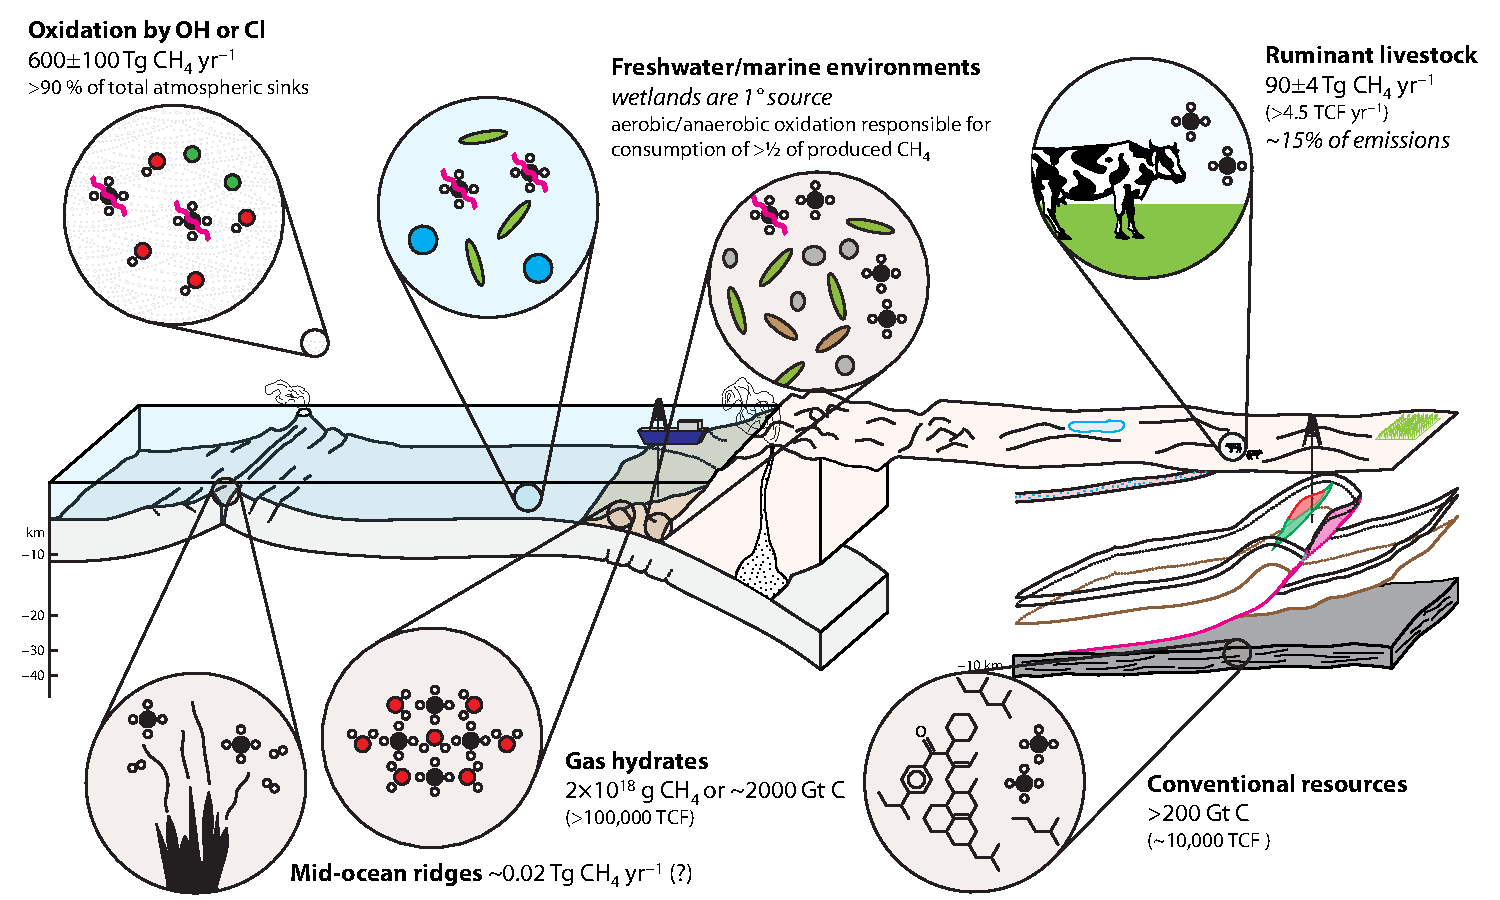
\includegraphics[width=0.95\textwidth]{figures/Fig1.1.pdf}
	\caption[Reservoirs and fluxes of CH\textsubscript{4} on Earth]{Some of the many reservoirs and fluxes of methane on
		Earth, and their relative magnitudes \parencite{Kvenvolden_1988_CG,Keir_2010_GRL,IPCC_AR5_WG1,Kirschke++_2013_NG}.}
	\label{fig:1:1}
\end{sidewaysfigure}

Methane is the simplest and most abundant hydrocarbon. \mrefs[]{Figure}{fig:1:1} shows some statistics on the
portions of the methane cycle that this thesis touches upon.

\section{Essential definitions}\label{sec:1:essential-definitions}


\begin{SCfigure*}
	\centering
	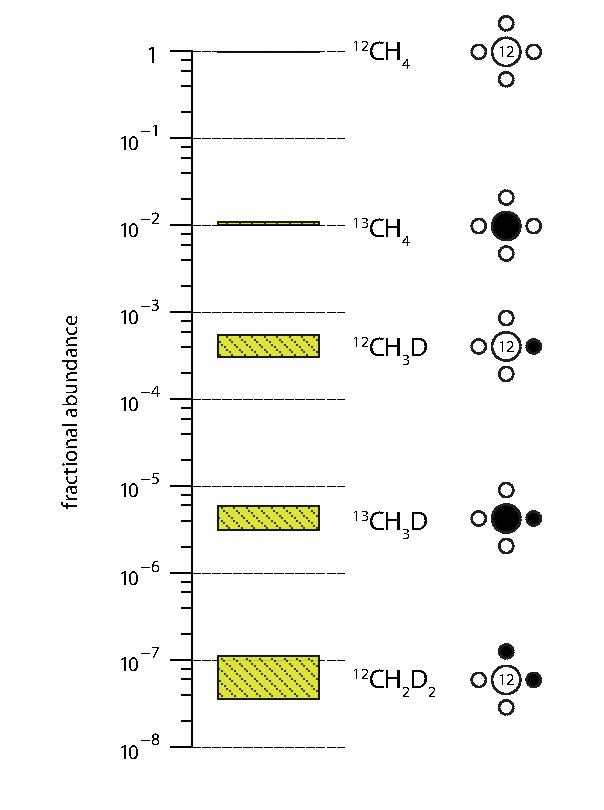
\includegraphics[width=0.52\textwidth]{figures/Fig1.2.pdf}
	\captionsetup{format=myformat}	% hrule beneath caption
	\caption[Natural abundances of methane isotopologues]{Relative abundance of the five most abundant methane
		isotopologues in nature.\protect\\}
	\label{fig:1:2}
\end{SCfigure*}


The \emph{isotopologues} (or isotopic homologues) of a compound have the
same elemental composition and chemical structure, but differ only in
the identity of the isotopes of one or more atoms. The word
\emph{isotopologue} is also seen as \emph{isotopolog}.

\sidecaptionvpos{figure}{t}	%typset sidecap at top
\begin{SCfigure*}
	\centering
	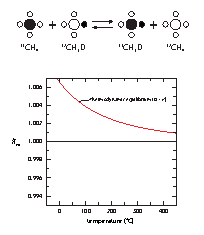
\includegraphics[width=0.52\textwidth]{figures/Fig1.3.pdf}
	\captionsetup{format=myregular}	% no hrule beneath caption
	\caption[Equilibrium constant for \textsuperscript{13}CH\textsubscript{3}D formation vs.\ temperature]{Temperature-dependence of the equilibrium constant for the
		isotopologue exchange reaction in \mrefs[]{Reaction}{eqn:1:exchange} (also shown graphically at
		top).}
	\label{fig:1:3}
\end{SCfigure*}
\sidecaptionvpos{figure}{b}	%reset to default


\begin{figure}
	\centering
	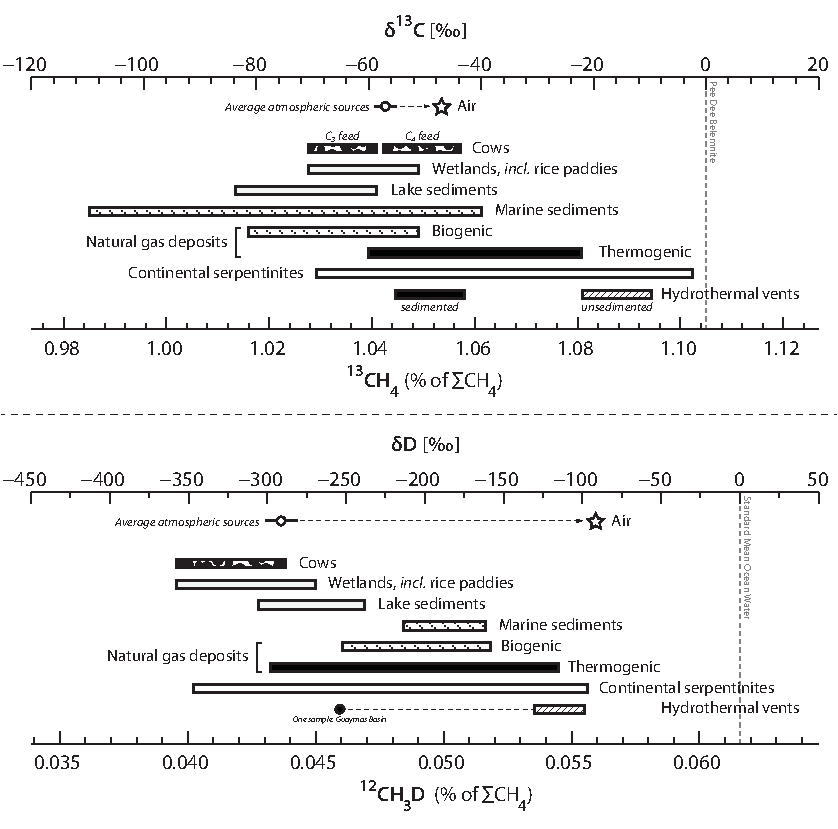
\includegraphics[width=0.75\textwidth]{figures/Fig1.NA.pdf}
	\captionsetup{format=myformat}	% hrule beneath caption
	\caption[Natural abundances of singly-substituted methane isotopologues]{Typical abundances of \textsuperscript{13}CH\textsubscript{4} (\textit{top}) and \textsuperscript{12}CH\textsubscript{3}D (\textit{bottom}) in nature.}
	\label{fig:1:NA}
\end{figure}


The goal of this thesis is to help map the distribution and behavior of
the four most abundant methane isotopologues at the Earth surface and in
the crustal subsurface. These isotopologues are shown in \mrefs[]{Figs.}{fig:1:2} and~\ref{fig:1:3} (approximate ranges of abundance for the singly-substituted methane isotopologues are 
shown in \autoref{fig:1:NA}) and
written in the isotope exchange reaction below:
\begin{equation}\label{eqn:1:exchange}
{}^{13}\text{CH}_4+ {}^{12}{\text{CH}}_3\text{D}\rightleftharpoons {}^{13}{\text{CH}}_3\text{D}+ {}^{12}{\text{CH}}_4
\end{equation}


\begin{SCfigure*}
	\centering
	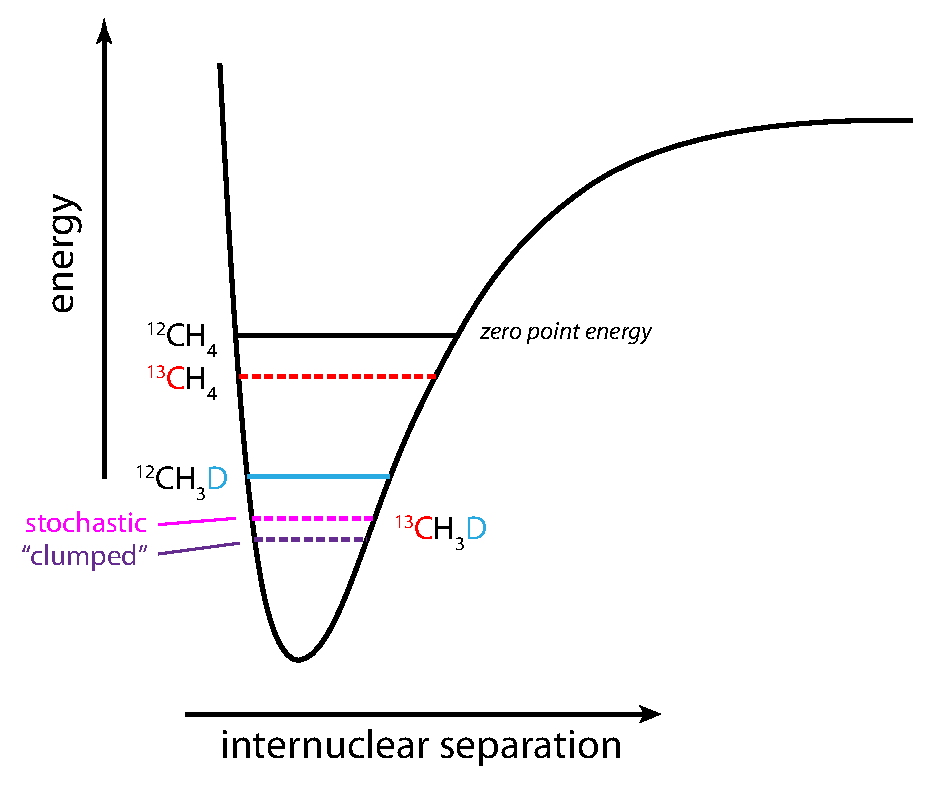
\includegraphics[width=0.55\textwidth]{figures/Fig1.4.pdf}
	\captionsetup{format=myformat}	% hrule beneath caption
	\caption[Statistical mechanical origin of preferential heavy-isotope clumping]{Zero-point energy lowering and the origin of non-stochastic clumped isotopologue composition
		at equilibrium.  The zero-point energy (the energy of the ground state, the quantum state with the lowest possible energy) of a molecule of methane is lowered upon substitution of heavy isotopes.  The amount by which the zero-point energy is lowered upon double-isotope substitution (e.g., \ce{^{12}CH4} to \ce{^{13}CH3D}) is slightly greater than the sum of the effects of substituting only one heavy isotope (to make \ce{^{13}CH4} and \ce{^{12}CH3D}).  This deviation from the ``rule of the geometric mean'' \parencite{Bigeleisen_1955_JCP} is particularly pronounced at lower temperatures, and is the origin of the preferential clumping at equilibrium shown in \autoref{fig:1:3}.  For a detailed treatment, readers are referred to \textcite{Eiler_2007_EPSL}.}
	\label{fig:1:4}
\end{SCfigure*}

In this reaction, one deuterium (D) is exchanged for one hydrogen (H),
while leaving in place the two different carbon (C) isotopes and the
three other H's to which each C is connected. The equilibrium constant
for this reaction is primarily a function of temperature (the
effect of pressure is negligible at near-surface conditions), and is
shown in \autoref{fig:1:3}. The equilibrium constant for this reaction
asymptotically approaches unity as temperatures increase towards
infinity. A sample of methane whose relative abundance of isotopologues
obey the relation
\cee{(\textsuperscript{13}CH\textsubscript{4})(\textsuperscript{12}CH\textsubscript{3}D)
=
(\textsuperscript{13}CH\textsubscript{3}D)(\textsuperscript{12}CH\textsubscript{4})}
(i.e., has a reaction quotient equal to unity) is said to have a
\emph{stochastic distribution} of isotopes among isotopologues. At
lower temperatures, the equilibrium constant is greater than one, albeit
only slightly, by 0.6\% or 6‰ (permil) at room temperature. The origin
of this \emph{clumpiness} at equilibrium at lower temperatures arises from a disproportionate lowering of zero-point energy upon clumping of two or more heavy isotopes (\autoref{fig:1:4}). For more on this topic, readers are referred to \textcite{Eiler_2007_EPSL}.



\begin{SCfigure*}
	\centering
	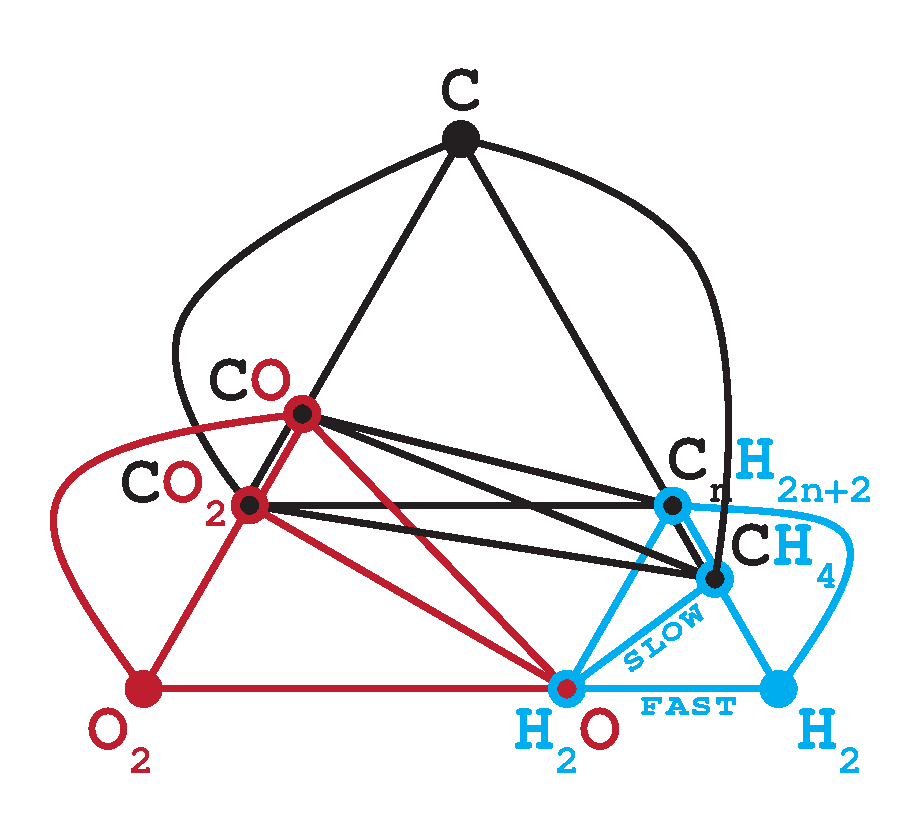
\includegraphics[width=0.4\textwidth]{figures/Fig1.5.pdf}
	\captionsetup{format=myformat}	% hrule beneath caption
	\caption[Pathways for isotopic exchange amongst C--O--H species]{Pathways for isotopic exchange between major species in
		the system C--O--H. The core \& ring of nodes with two colors represent
		the central \& outer atoms, respectively. Each line in this diagram
		represents a geothermometer comprising the isotope ratios of the
		corresponding element in the species at the nodes connected by the line. (Not shown:
		H\textsubscript{3}COOH, H\textsubscript{2}CO, CH\textsubscript{3}OH)}
	\label{fig:1:5}
\end{SCfigure*}

Attainment of equilibrium in CH\textsubscript{4} clumped isotopologue
abundances requires reordering of the C--H bonds within molecules. This
may occur by homogeneous (direct) exchange of H between two
CH\textsubscript{4} molecules, or by all CH\textsubscript{4} molecules
independently exchanging H with a second species (heterogeneous).
Understanding the mechanisms enabling exchange in various environments
is vital for correct interpretation of classical and novel stable
isotope geothermometers. \mrefs[]{Figure}{fig:1:5} shows the many pathways by which
several single-carbon compounds can exchange isotopes with compounds in
the C--O--H system.

\section{Preview of thesis content}\label{preview-of-thesis-content}

Several labs are now able to make measurements of the reaction quotient
of \mrefs{Reaction}{eqn:1:exchange}, to better than 0.05\% (or 0.5‰). These include John
Eiler's lab at Caltech \parencite{Stolper++_2014_GCA}, Shuhei Ono's lab at MIT
\parencite{Ono++_2014_AC}, and Ed Young's lab at UCLA \parencite{Young++_2016_IJMS}. For
those interested in the race towards measuring intact methane
isotopologues, readers are referred to \textcite{Jones_2012_Earth}.

\mrefs[]{Chapters}{ch:2}, \ref{ch:3}, and \ref{ch:4} and \autoref{dx:A} describe insights we have gleaned
while studying the origin of C, H, and carbon-hydrogen bonds in
CH\textsubscript{4} using measurements and models of the abundance and
behavior of methane isotopologues. \autoref{ch:2} presents the first survey
of the abundance of fully-resolved
\textsuperscript{13}CH\textsubscript{3}D in various environments on
Earth, and shows how and why microbial methanogenesis occurring under
high H\textsubscript{2} and low CO\textsubscript{2} levels might leave a
very distinct record in the isotopic composition of the
CH\textsubscript{4} produced (\autoref{fig:1:6}). \autoref{ch:2} also briefly touches on
a potential for hydrogen exchange observed in high-maturity thermogenic
gases.

\begin{SCfigure*}
	\centering
	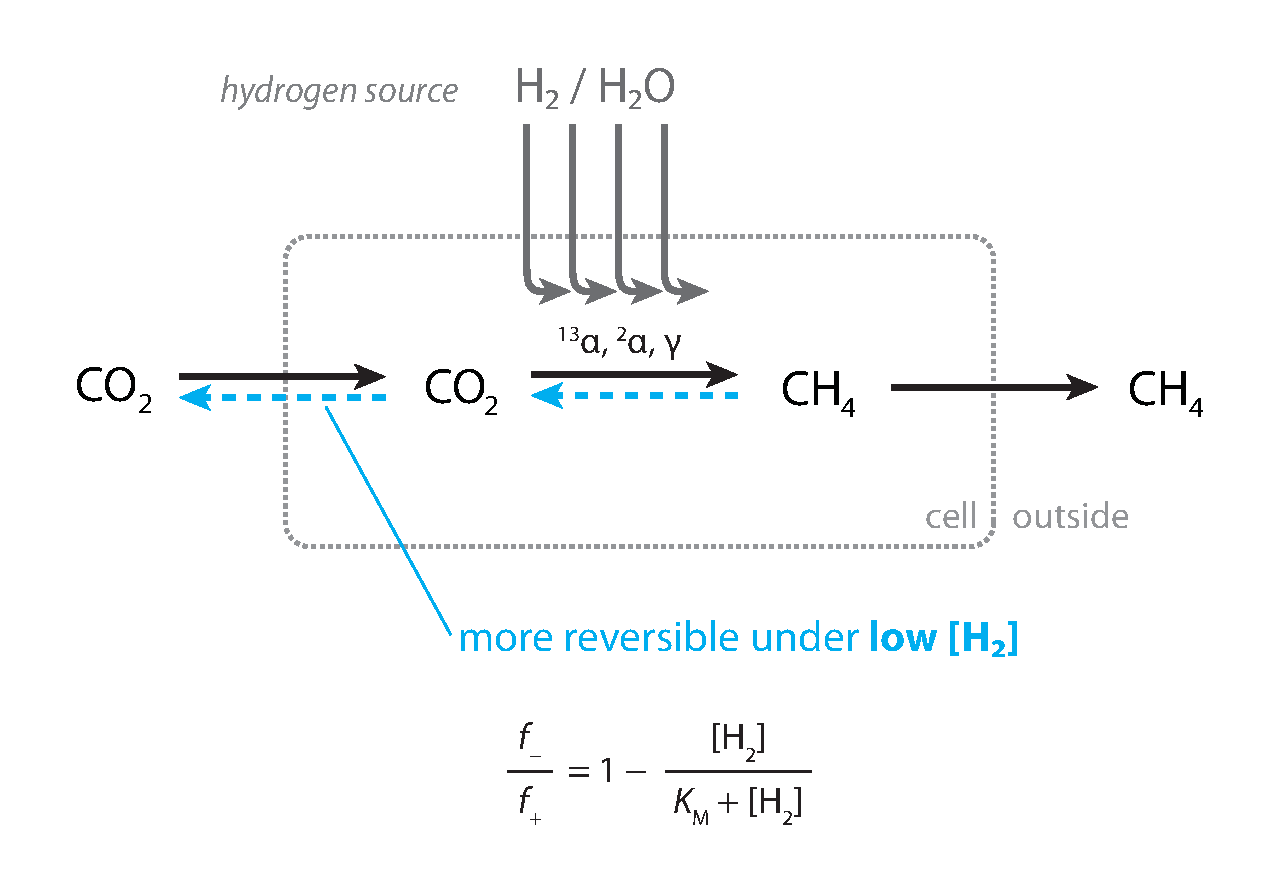
\includegraphics[width=0.6\textwidth]{figures/Fig1.6.pdf}
	\captionsetup{format=myformat}	% hrule beneath caption
	\caption[{Control of methane isotopologue abundances by reversibility and [H\textsubscript{2}] during methanogenesis}]{Preview of one of the main conclusions of \autoref{ch:2}:
		The isotopic composition of methane produced by methanogenesis is
		determined by reversibility, which in turn is related to free energy
		(for which the primary variable in most environments is H\textsubscript{2}
		concentration).}
	\label{fig:1:6}
\end{SCfigure*}

\begin{sidewaysfigure}
	\centering
	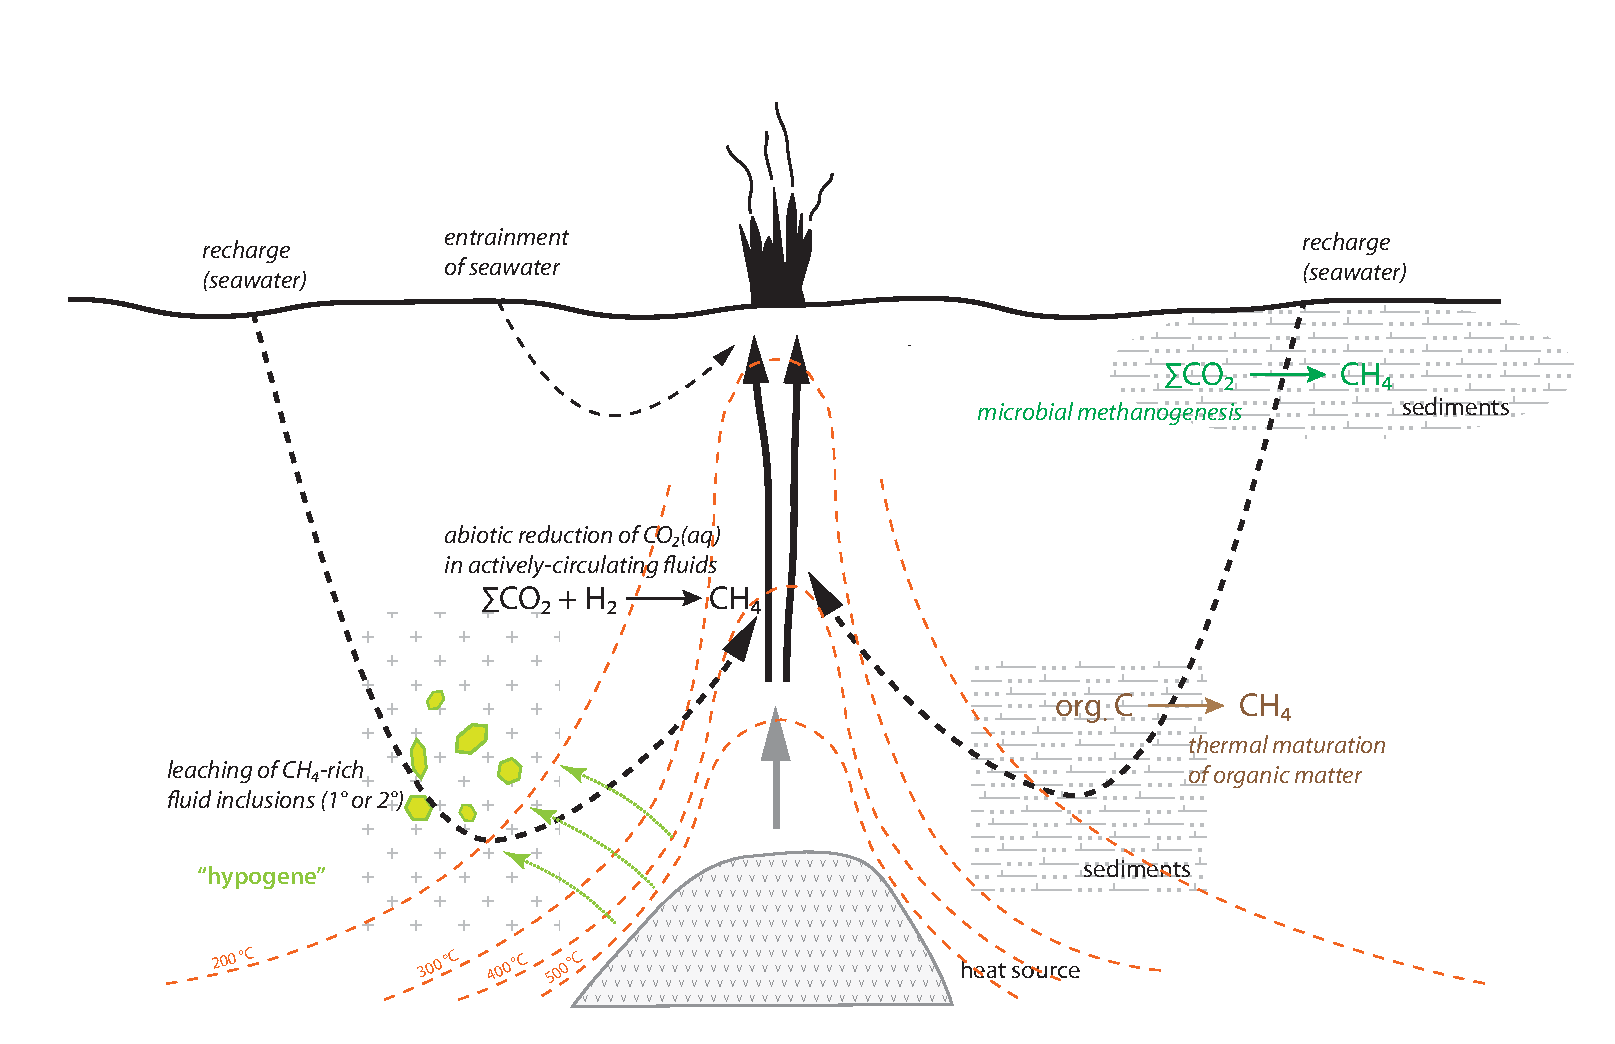
\includegraphics[width=0.95\textwidth]{figures/Fig1.7.pdf}
%	\captionsetup{format=myformat}	% hrule beneath caption
	\caption[Possible origins of methane at oceanic spreading centers]{Pathways for methane formation in mid-ocean ridge
		hydrothermal systems. \autoref{ch:3} shows how data from sediment-poor
		systems are most compatible with what we term a \emph{hypogene} origin
		for methane in vent fluids at oceanic spreading centers.}
	\label{fig:1:7}
\end{sidewaysfigure}

\autoref{ch:3} presents a study that attempts to address the oft-contentious
question of where and how methane in seafloor hydrothermal systems
forms. A diagram showing the several main proposed avenues for methane
formation in such systems is in \autoref{fig:1:7}. There is interest in knowing the
answer to this question because of potential implications for the origin
of life at deep-sea hot springs.

\autoref{ch:4} is an experimental and theoretical study that illustrates how
one major sink of methane in the environment, aerobic methanotrophy,
affects the isotopologue abundances of leftover methane (\autoref{fig:1:8}). The
results and equations can be generalized to other major methane sinks \parencite[including oxidation by OH and Cl in the atmosphere;][]{Whitehill++_2017_GCA}, and to other isotopologues (e.g.,
\textsuperscript{12}CH\textsubscript{2}D\textsubscript{2}).


\begin{SCfigure*}
	\centering
	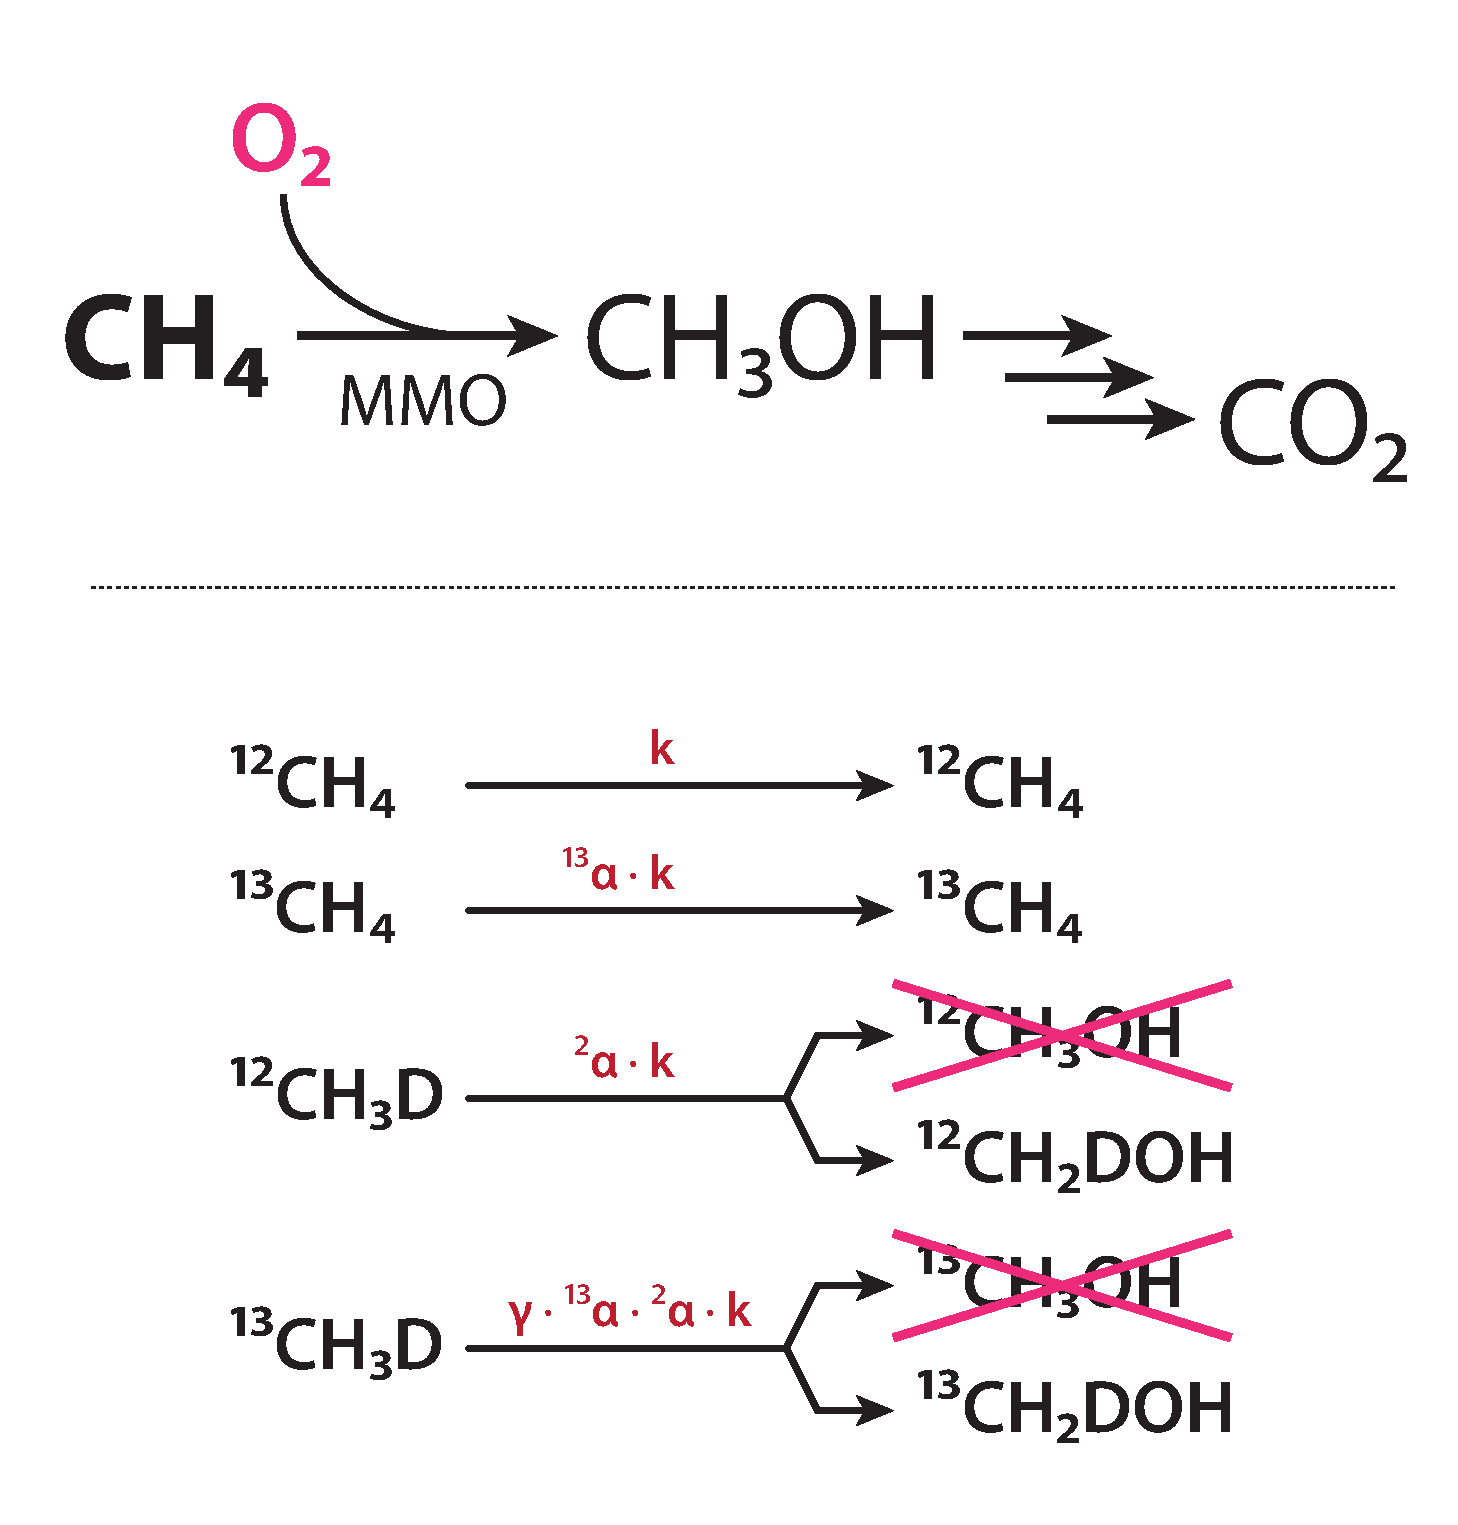
\includegraphics[width=0.45\textwidth]{figures/Fig1.8.pdf}
	\captionsetup{format=myformat}	% hrule beneath caption
	\caption[Reaction scheme for four stable isotopologues of methane during methane oxidation]{Reaction scheme for four stable isotopologues of
		methane during methane oxidation. Abstraction of D is
		\textasciitilde{}100× slower than H-abstraction. Substitution of D at an
		adjacent site has a small (\textasciitilde{}10\%)
		effect \parencite{Nesheim+Lipscomb_1996_Bc}. This means that
		the D/H fractionation comes mostly from the ¾ probability associated
		with abstraction of H from monodeuterated methane. 
		
		\quad \autoref{ch:4} and \textcite{Whitehill++_2017_GCA} show that
		fractionations are related by: 	\cee{\textsuperscript{13}CH\textsubscript{3}D/\textsuperscript{12}CH\textsubscript{4}
		= $\gamma$ × (\textsuperscript{13}C/\textsuperscript{12}C) × (D/H)},  where $\gamma$ is
		a number close to 1.000 (identical within error for OH and aerobic
		methanotrophy, and slightly less than 1 for Cl). Together, these
		fractionation factors constrain the effects on
		\textsuperscript{13}CH\textsubscript{3}D by the major methane sink
		reactions in the atmosphere and in oxic microbial habitats on Earth.}
	\label{fig:1:8}
\end{SCfigure*}

\begin{SCfigure*}
	\centering
	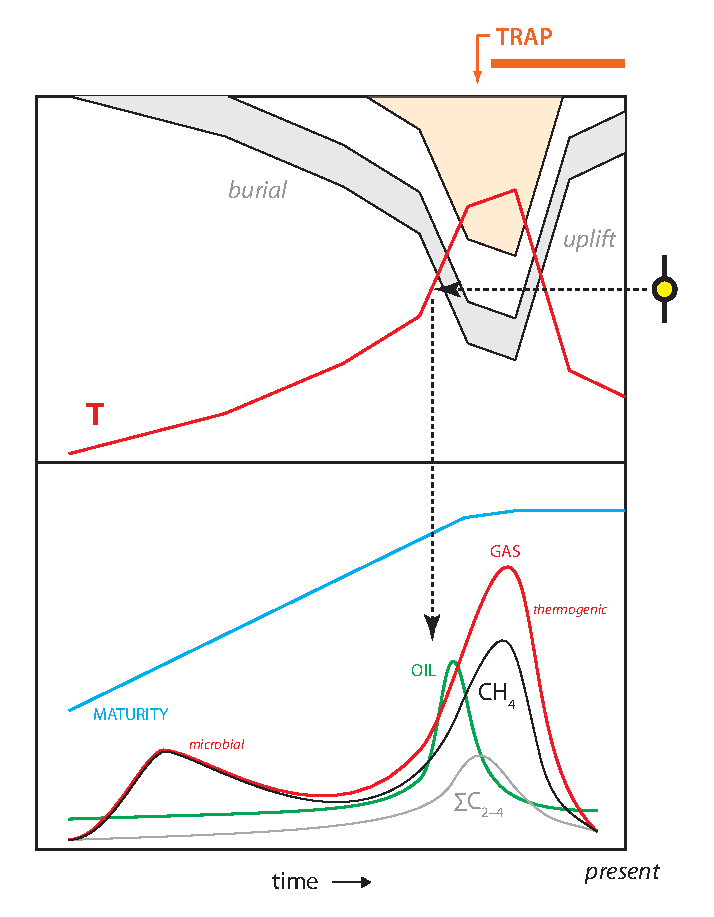
\includegraphics[width=0.6\textwidth]{figures/Fig1.9.pdf}
	\captionsetup{format=myformat}	% hrule beneath caption
	\caption[Petroleum system applications of
	\textsuperscript{13}CH\textsubscript{3}D]{Petroleum system applications of
		\textsuperscript{13}CH\textsubscript{3}D. The potential application
		space of methane isotopologue geothermometry and geospeedometry include
		the ability to link key hydrocarbon system elements (particularly
		elements of source, charge, and trap) in time and space, to calibrate
		and/or validate basin model predictions and coupled source rock
		maturation simulations, and to define a new metric of maturity based
		solely on fluid chemistry.}
	\label{fig:1:9}
\end{SCfigure*}

Research on the behavior of methane isotopologues like
\textsuperscript{13}CH\textsubscript{3}D have a natural alignment to
many of the questions that are important and possibly unanswered in
assessment of petroleum systems, particularly in poorly understood
basins (\autoref{fig:1:9}). In particular, measurements of methane isotopologues can
\begin{itemize}
	\item
	place quantitative constraints on the stability and origin of C--H
	bonds in hydrocarbons in the Earth's subsurface;
	\item
	test interpretive models of natural gas composition and gas isotope
	systematics; and
	\item
	be used to help anchor the chemistry of natural gases to time and
	temperature.
\end{itemize}

\mrefs[]{Appendices}{dx:A} and \ref{dx:B} represent some initial efforts to read the
hydrogen-isotope and clumped isotopologue record of natural gases and
define what those records mean.

\autoref{dx:C} offers miscellaneous tricks, tips, and data that didn't fit
anywhere else.

























